\subsubsection{Purpose}
Any user is encouraged to subscribe through the web application or the mobile one. The system provides the user the possibility to become a registered user by filling a registration form or directly accessing through third-party accounts like Google or Facebook. After authenticating, functionalities concerning the account management are also provided, so the user can easily:
\begin{enumerate}
	\item Login into his/her account.
    \item Recover forgotten password by resetting it
    \item Update account data.
\end{enumerate}
Users are simply asked to insert this information:
\begin{itemize}
	\item E-mail address
	\item Username
	\item Password
    \item Name
    \item Surname

\end{itemize}
Some basic checks are performed when the user is asked to fill the form in order to register. For instance, the system requires the user to insert a password that contains at least one number, one capital letter and a symbol, whose length is not less than 8 characters. The user will be asked to insert the password twice. Clearly, if the privacy policy and terms of condition are not authorized, the subscription is nullified. The user is free to delete his account at any time. Credentials are encrypted stored in the device so that the user must never insert them but the first time. Whilst asking for registration and logging in to access the application can be seen as a waste of time, it is designed for allowing the user to manage his/her own reminders and events both from the mobile and the web application so that they are always synchronized.
\subsubsection{Scenario 1}
Alice decides to give the application a try, so, after downloading and launching it, she is displayed a login page where she is asked to sign up in order to access to all its services. She immediately notices the Google logo and, to avoid wasting time by creating another account, she decides to sign up with Google. Everything goes well, and she is welcomed by the user-friendly interface and the application is now fully working.
\subsubsection{Scenario 2}
Bob accesses Travlendar+ application through the web page and clicks on the \textit{Login} button. He is asked to enter his username and password, but figures out that he had never joined to the service before, so he goes back and decides to sign up. Being completely new, he creates a totally new account. When filling the form, he inputs \textit{Bob} as username. Turns out that this username has already been used so Bob is warned that that username is unavailable. He changes username, continues fulfilling the form and eventually, a window welcomes him by starting a little demo which guides him around the website. He is also informed that to fully access the application he must confirm the evidence of the registration by clicking the link sent via email.

\subsubsection{Use case}
The use case for user registration is shown in Table \ref{usecase-login}, whereas the use case for user login is shown in Table \ref{usecase-registration}.
\begin{table}
\centering
\begin{tabular}{|c||p{0.6\textwidth}|}
	\hline
    Name & Login \\ \hline
    Goal & G1 \\ \hline
    Actors & Registered User \\ \hline
    Assumptions & \begin{itemize}
    					\item The user has already signed up into the system. 
                        \item The user is not logged into the system yet.
                  \end{itemize} \\ \hline
    Events flow & \begin{enumerate}
                   		\item The user opens the \textit{login page} of the system;
                        \item The user types in username and password.
                        \item The system recognizes the identity and ensures that the user who is logging it is who he claims to be.
                        \item The user can visualize his personal calendar and access to the system's functionalities provided to him.
                     \end{enumerate} \\ \hline
   Exit conditions & The user is now logged into the system. \\ \hline
   Exceptions & The \textit{username and password} inserted are wrong, an error message is shown. The user is not logged.\\ \hline
\end{tabular}
\caption{Use case for user login.}
\label{usecase-login}
\end{table}

\begin{table}
\centering
\begin{tabular}{| l | p{0.6\textwidth} |}
\hline
Name & Registration \\ \hline
Actor & Unregistered user \\ \hline
Goal & G0 \\ \hline
Input condition & The user creates a new user account or signs up with third-party accounts. \\ \hline
Events flow & \begin{enumerate}
	\item The user decides whether he/she wants to create a completely new account or to undergo an application-based enrollment.
	\item Either the user is redirected to the third-party sign-up page and asked to insert his/her credentials or a registration form is loaded and the user is asked to compile it.\label{load-registration}
	\item In both cases, the user is asked to authorize the privacy policy and terms of conditions.
	\item If the user decided to create a new account, then he/she can confirm the registration by accepting the linked sent via email. No two-factor authentication is called for.
	\end{enumerate}
\\
\hline
Output condition & The system welcomes the user by informing him/her that the registration was done successfully. \\
\hline

Exception &  \begin{itemize}
	\item If username or similar data are already been taken or invalid username is provided, the user is warned to choose for a different username.
   	\item If no account exists when signing up through third-party services, they will also handle resulting possible errors.
	\end{itemize}
 \\ \hline
\end{tabular}
\caption{Use case for user registration.}
\label{usecase-registration}
\end{table}

\subsubsection{Sequence diagram}
The sequence diagram of the login process is illustrated in Figure \ref{fig:SequenceLogin}.
\begin{figure}
	\centering
	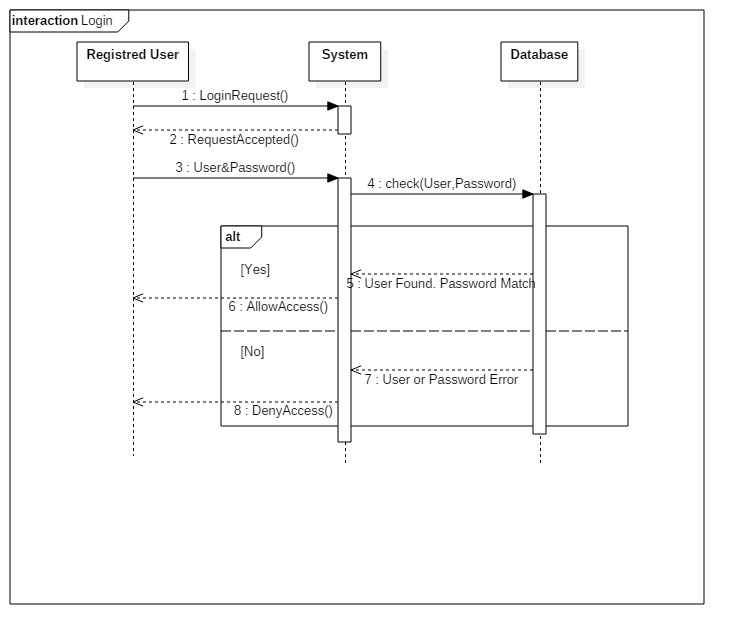
\includegraphics[width=6in]{./diagrams/SequenceLogin.png}
	\caption{Sequence Diagram: Login.}
	\label{fig:SequenceLogin}
\end{figure}

\subsubsection{Statechart}
The statechart of the registration process is illustrated in Figure \ref{fig:StatechartLogin}.
\begin{figure}
	\centering
	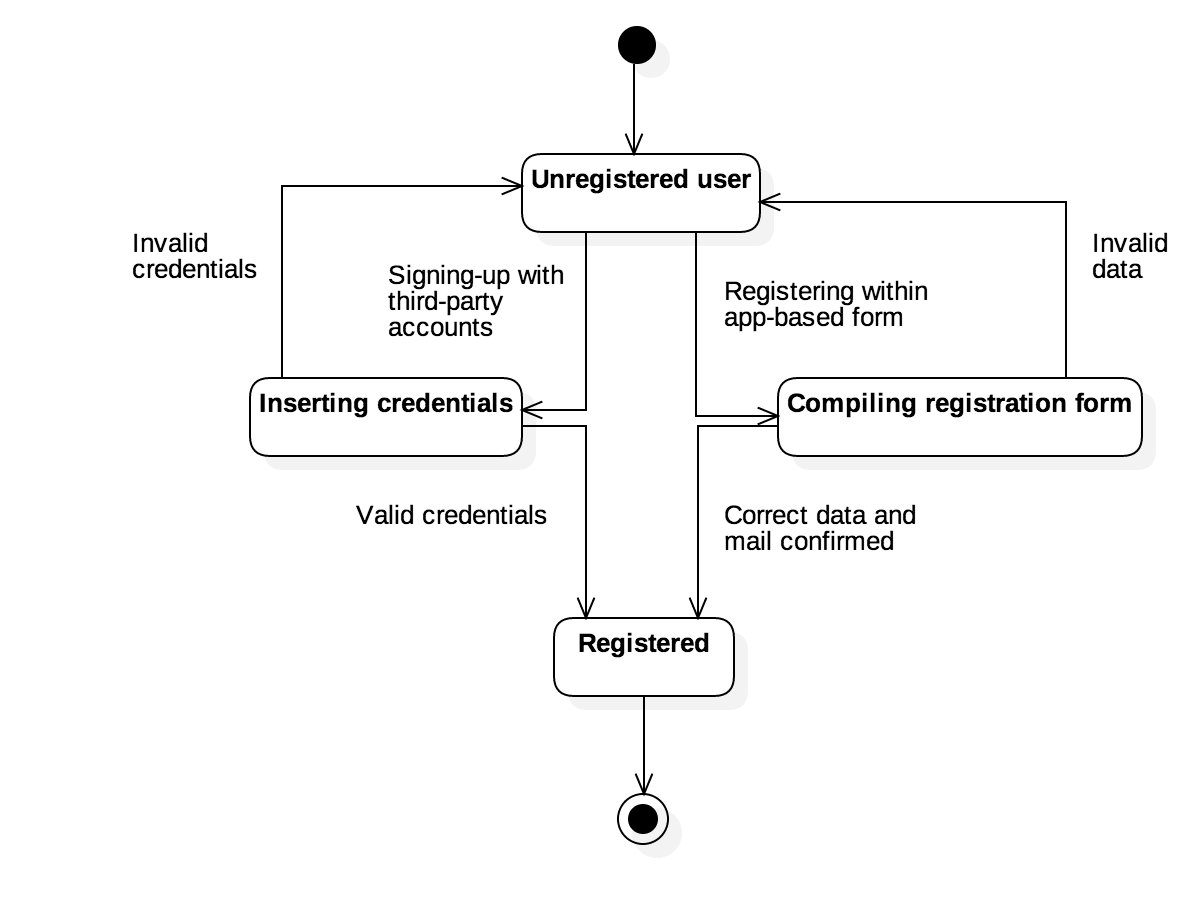
\includegraphics[width=6in]{./diagrams/StatechartLogin.png}
	\caption{Statechart Diagram: Login.}
	\label{fig:StatechartLogin}
\end{figure}

\subsubsection{Mockup}
The mockup of the login interface is show in Figure \ref{fig:MockupLogin}.
\begin{figure}
	\centering
	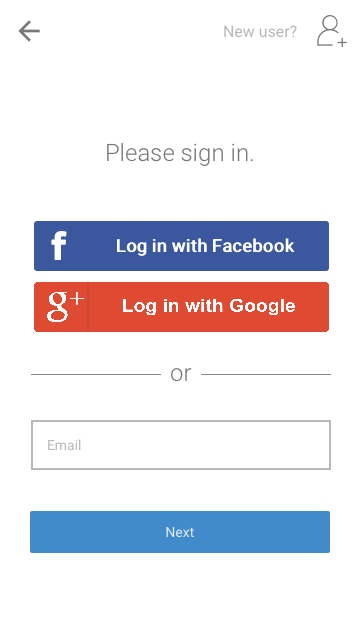
\includegraphics[width=4.5in]{./images/login.png}
	\caption{Login mockup.}
	\label{fig:MockupLogin}
\end{figure}